\section{Auswertung}
\label{sec:Auswertung}
Zuerst wurde die Untergrundrate mit einem Messintervall $t=\SI{300}{\second}$ ermittelt. 
Die Messwerte finden sich in der \autoref{tab:untergrund}.
\subsection{Vanadium}
Bei der Vanadiumprobe wurde in Zeitabständen von $\increment t = \SI{30}{\second}$ die in den Zeitabschnitten aufgenommenen Impulse notiert. 
Die Messwerten lassen sich in \autoref{tab:vanadium} finden. 
Die Untergrundrate für  dieses Messintervall ergibt sich zu:
\begin{equation*}
  N_{\text{U}, \SI{30}{\second}} = \num{13.9 \pm 0.4}
\end{equation*}
\begin{figure}
  \centering
  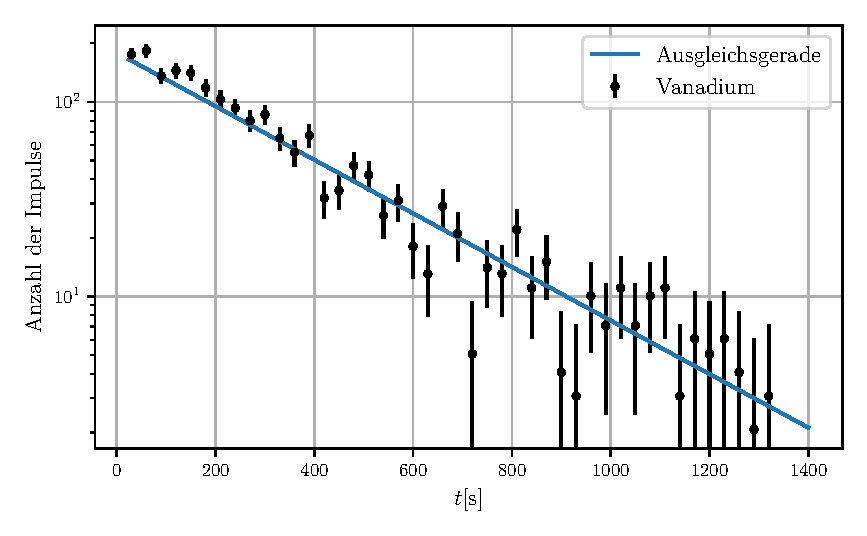
\includegraphics{build/vanadium.pdf}
  \caption{Die Messwerte der Vanadiumprobe mit einer linearen Ausgleichsgeraden in einem Halblogarithmischen Diagramm.}
  \label{fig:vana1}
\end{figure}
Die durch die Untergrundrate bereinigten Messwerte wurden anschließend in einem $t$-$N$-Diagramm halblogarithmisch aufgetragen.
Dies ist in der \autoref{fig:vana1} zu finden. 
Außerdem wurde eine Ausgleichrechnung mit python der Form $\log(N) = a\cdot t + c$ durchgeführt.
Die Parameter ergeben sich zu :
\begin{align*}
  a &= \SI{-1.38(70)e-3}{\per\second}\\
  c &= \num{2.25\pm 0.06}
\end{align*}
Damit die Halbwertszeit ausgerechent werden kann, müssen die Parameter von der dekadisch logarithmischen Darstellung in die natürliche Basis umgerechnet werden.
In der natürlichen Basis lauten diese dann:
\begin{align*}
  a &= \SI{-3.17(16)e-3}{\per\second}\\
  c &= \num{5.19 \pm 0.13}
\end{align*}
Mit \eqref{eqn:halbwertszeit} ergibt sich die Halbwertszeit von Vanadium zu:
\begin{equation*}
  T = \frac{\ln(2)}{\lambda} = \SI{219\pm 11}{\second}
\end{equation*}
\\
Da die letzten Zeitintervalle geringe Zählraten haben, werden die Messwerte von Vanadium bis $t=\SI{450}{\second}$ nochmale geplottet und mit einer Funktion der Form $\log(N) = a\cdot t +c $ genähert.
Die Ausgleichsrechnung erfolgt mit python und ergibt in der dekadisch logarithmischen Darstellung:
\begin{align*}
  a &= \SI{-1.67(13)e-3}{\per\second}\\
  c &= \num{2.35 \pm 0.04}
\end{align*}
Dies ist in geplottet in der \autoref{fig:vana2}.
\begin{figure}
  \centering
  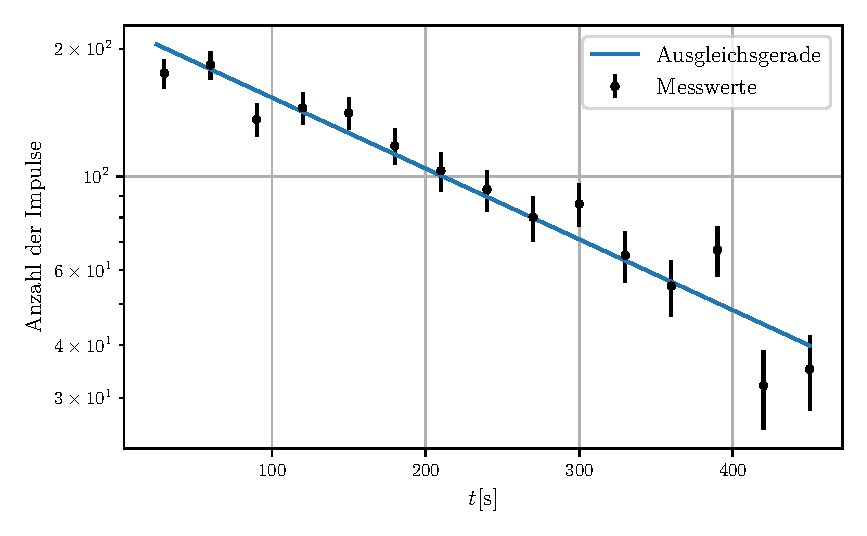
\includegraphics{build/vana2.pdf}
  \caption{Die Messwerte der Vanadiumprobe bis zur vorher ausgerechneten doppelten Halbwertszeit in einem halblogarithmischen Diagramm.}
  \label{fig:vana2}
\end{figure}
Nach der Umrechnung in die natürliche Basis folgt für die Ausgleichsrechnung:
\begin{equation*}
  \ln(N) = (\SI{-3.85(31)e-3}{\per\second}) \cdot t + (\num{5.42 \pm 0.08})
\end{equation*}
Somit errechnet sich die Halbwertszeit nach \eqref{eqn:halbwertszeit} bei dieser Auswahl der Messwert zu:
\begin{equation*}
  T = \SI{180 \pm 14}{\second}
\end{equation*}

\subsection{Rhodium}
Die Rhodiumprobe wurde mit einem Messintervall von $t= \SI{15}{\second}$ ausgemessen, so dass sich die Untergrundrate zu 
\begin{equation*}
  N_{\text{U}, \SI{15}{\second}} = \num{6.96\pm 0.19}
\end{equation*}
ergibt.
Die Messwerte der Rhodiumprobe, sowie die um die Untergrundrate bereinigten Messwerte sind in der \autoref{tab:rhodium} zu finden.
Anschließend wurden die Messwerte halblogarithmisch in ein Diagramm aufgetragen, siehe \autoref{fig:rhodium} .
\begin{figure}
  \centering
  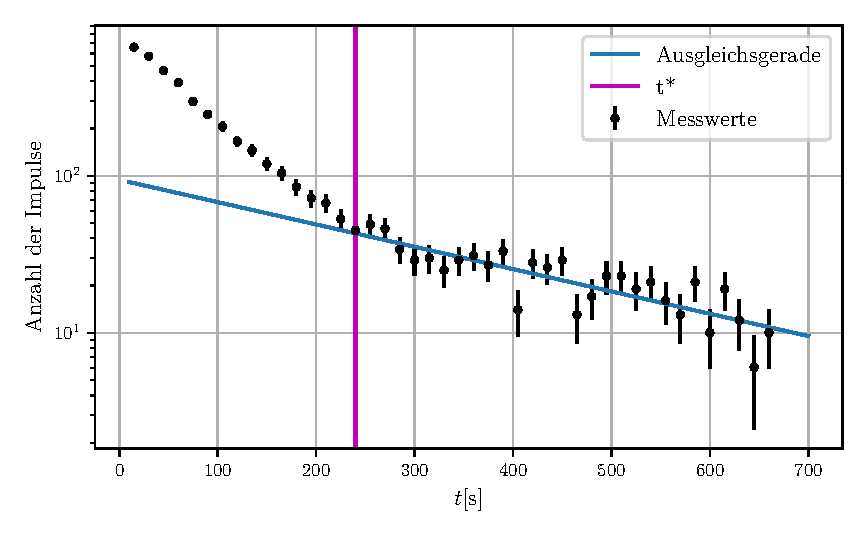
\includegraphics[width=\textwidth]{build/rhodium.pdf}
  \caption{Die Messwerte von Rhodium mit einer Ausgleichsrechnung für den langlebigen Zerfall in einem halblogarithmischen Diagramm.}
  \label{fig:rhodium}
\end{figure}
Da Rhodium in $\ce{^{104\text{i}}Rh}$ und $\ce{^{104}Rh}$ zerfällt, wird zuerst der langlebige Zerfall betrachten.
Der Zeitpunkt, in dem nur noch der langlebiger Zerfall vorliegt, wurde in \autoref{fig:rhodium} zu $t^* = \SI{240}{\second}$ bestimmt. 
Für die darauf folgenden Werte wurde eine Ausgleichsrechnung der Form $\log(N) = a \cdot t + c $ mit python druchgeführt. 
Die Parameter ergeben sich zu: 
\begin{align*}
  a &= \SI{-1.42(17)e-3}{\per\second}\\
  c &= \num{1.97 \pm 0.08}
\end{align*}
Nachdem die Steigung in die die natürliche Basis umgerechnet wurde, lautet die lineare Abbildung
\begin{equation} \label{eqn:ln_rho_lang}
  \ln(N) = \SI{-3.3(4)e-3}{\per\second} \cdot t + (\num{4.55 \pm 0.19})
\end{equation}
und die Halbwertszeit für den langlebigen Zerfall berechnet sich nach \eqref{eqn:halbwertszeit} zu:
\begin{equation*}
  T_{\text{H}, l} = \SI{212 \pm 26}{\second}
\end{equation*}
Die Zerfallsrate für den langlebige Zerfall von Rhodium lautet somit:
\begin{equation*}
  N_{\increment \text{t}, \text{lang}}(t) = (\num{-4.7 \pm 1.1})\cdot \exp((\num{0.0033 \pm 0.0004})t)
\end{equation*}
\\
Zur Betrachtung des kurzlebigen Zerfalls wird nun die Zerfallsrate des langlebigen Zerfalls von der Gesamtanzahl für Zeiten bis $t = \SI{210}{\second}$ abgezogen.
Diese Werte wurden halblogarithmisch in ein Diagramm getragen (siehe \autoref{fig:rhodium_kurz}) und mit einer Funktion der Form $\log(N) = a \cdot t + c$ angenähert.
\begin{figure}[H]
  \centering
  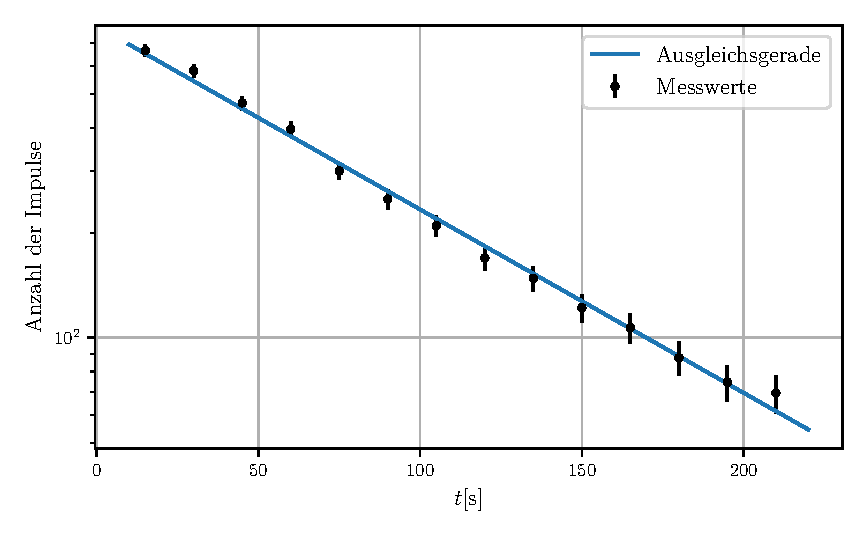
\includegraphics[width=\textwidth]{build/rhodium_kurz.pdf}
  \caption{Zur Ermittlung der Halbwertszeit des kurzlebigen Zerfalls von Rhodium wurden die Differenz der um die Untergrundrate bereinigten Messwerte und der für diesen Zeitpunkt berechneten Zerfallsrate des langlebigen Zerfalls gegen die Zeit aufgetragen.}
  \label{fig:rhodium_kurz}
\end{figure}
Die Ausgleichsgerade wurde mit python ermittelt und lautet in dekadisch logarithmischer Darstellung:
\begin{align*}
  a &= \SI{-5.26(11)e-3}{\per\second}\\
  c &= \num{2.893 \pm 0.014}
\end{align*}
In der natürlichen Basis lässt sich die Ausgleichsgerade so schreiben:
\begin{equation} \label{eqn:ln_rho_kurz}
  \ln(N) = (\SI{-0.01210\pm 0.00025}{\per\second})\cdot t + (\num{6.661\pm 0.032})
\end{equation}
Damit berechnet sich die Halbwertszeit des kurzlebigen Zerfalls nach \eqref{eqn:halbwertszeit} zu:
\begin{equation*}
  T_{\text{H},\text{k}}= \SI{57.3\pm 1.2}{\second}
\end{equation*}
Abschließend sind in der \autoref{fig:rhodium_ges} die Messwerte der Rhodiumprobe neben der Ausgleichsgeraden für den langlebigen Zerfall \eqref{eqn:ln_rho_lang}, für den kurzlebigen Zerfall \eqref{eqn:ln_rho_kurz} und deren Summe in einem halblogarithmischen $t$-$N$-Diagramm abgebildet.
\begin{figure}[H]
  \centering
  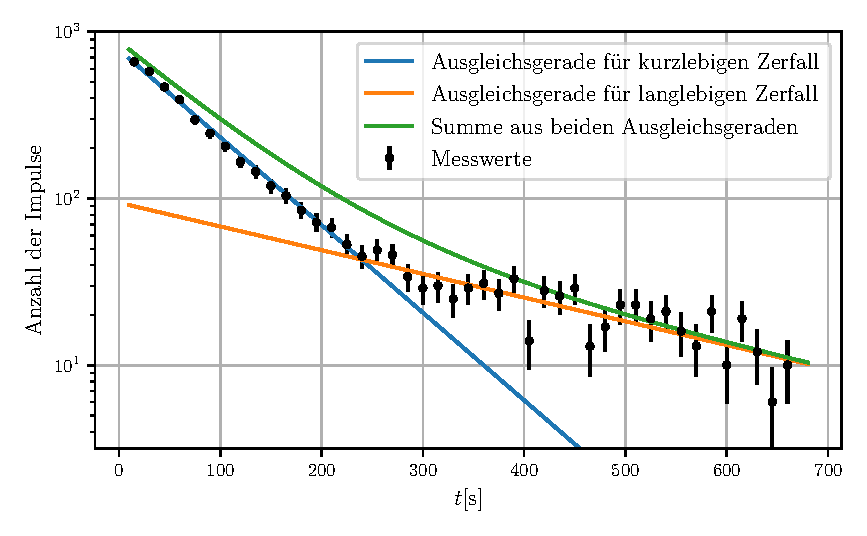
\includegraphics[width=\textwidth]{rhodium_ges.pdf}
  \caption{Die Messwerte der Rhodiumprobe sowie die einzelnen Ausgleichsgeraden und deren Summe in einem halblogrithmischen Diagramm.}
  \label{fig:rhodium_ges}  
\end{figure}

\subsection{Messwerte}
Die Messwerte der einzelnen Proben sind jeweils angegeben und zusätzlich die mit der Untergrundrate bereinigten Impulszahl inklusive der Messunsicherheit.
\begin{table}
  \centering
  \caption{Die Werte der Messung zur Untergrundrate.}
  \label{tab:untergrund}
  \begin{tabular}{S[table-format=4]
                  S[table-format=3]}
  \toprule
  {$t [\si{\second}]$}&{$N_{\text{U}}$}\\
  \midrule
  300 & 129 \\
  600 & 143 \\
  900 & 144 \\
  1200 & 136 \\
  1500 & 139 \\
  1800 & 126 \\
  2100 & 158 \\
  \bottomrule
  \end{tabular}
\end{table}

\begin{table}
  \centering
  \caption{Die gemessenen Impulszahlen der Vanadiumprobe.}
  \label{tab:vanadium}
  \begin{tabular}{S[table-format=4.1] %dt
                  S[table-format=3.1] %Nges
                  S[table-format=3.1] %N
    @{${}\pm{}$}  S[table-format=2.4]} %DN
  \toprule
  {$t [\si{\second}]$}&{$N_{\text{gemessen}}$}& \multicolumn{2}{c}{$N$}\\
  \midrule
30.0 & 189.0 & 175.1 & 13.2325\\
60.0 & 197.0 & 183.1 & 13.5314\\
90.0 & 150.0 & 136.1 & 11.6662\\
120.0 & 159.0 & 145.1 & 12.0457\\
150.0 & 155.0 & 141.1 & 11.8786\\
180.0 & 132.0 & 118.1 & 10.8674\\
210.0 & 117.0 & 103.1 & 10.1538\\
240.0 & 107.0 & 93.1 & 9.6488\\
270.0 & 94.0 & 80.1 & 8.9499\\
300.0 & 100.0 & 86.1 & 9.2790\\
330.0 & 79.0 & 65.1 & 8.0685\\
360.0 & 69.0 & 55.1 & 7.4229\\
390.0 & 81.0 & 67.1 & 8.1915\\
420.0 & 46.0 & 32.1 & 5.6657\\
450.0 & 49.0 & 35.1 & 5.9245\\
480.0 & 61.0 & 47.1 & 6.8629\\
510.0 & 56.0 & 42.1 & 6.4885\\
540.0 & 40.0 & 26.1 & 5.1088\\
570.0 & 45.0 & 31.1 & 5.5767\\
600.0 & 32.0 & 18.1 & 4.2544\\
630.0 & 27.0 & 13.1 & 3.6194\\
660.0 & 43.0 & 29.1 & 5.3944\\
690.0 & 35.0 & 21.1 & 4.5935\\
720.0 & 19.0 & 5.1 & 2.2583\\
750.0 & 28.0 & 14.1 & 3.7550\\
780.0 & 27.0 & 13.1 & 3.6194\\
810.0 & 36.0 & 22.1 & 4.7011\\
840.0 & 25.0 & 11.1 & 3.3317\\
870.0 & 29.0 & 15.1 & 3.8859\\
900.0 & 18.0 & 4.1 & 2.0249\\
930.0 & 17.0 & 3.1 & 1.7607\\
960.0 & 24.0 & 10.1 & 3.1780\\
990.0 & 21.0 & 7.1 & 2.6646\\
1020.0 & 25.0 & 11.1 & 3.3317\\
1050.0 & 21.0 & 7.1 & 2.6646\\
1080.0 & 24.0 & 10.1 & 3.1780\\
1110.0 & 25.0 & 11.1 & 3.3317\\
1140.0 & 17.0 & 3.1 & 1.7607\\
1170.0 & 20.0 & 6.1 & 2.4698\\
1200.0 & 19.0 & 5.1 & 2.2583\\
1230.0 & 20.0 & 6.1 & 2.4698\\
1260.0 & 18.0 & 4.1 & 2.0249\\
1290.0 & 16.0 & 2.1 & 1.4492\\
1320.0 & 17.0 & 3.1 & 1.7607\\
  \bottomrule
  \end{tabular}
\end{table}

\begin{table}
  \centering
  \caption{Die gemessenen Impulszahlen der Rhodiumprobe.}
  \label{tab:rhodium}
  \begin{tabular}{S[table-format=3.1] %dt
                  S[table-format=3.1] %Nges
                  S[table-format=3.2] %N
    @{${}\pm{}$}  S[table-format=2.4]} %DN
  \toprule
  {$t [\si{\second}]$}&{$N_{\text{gemessen}}$}& \multicolumn{2}{c}{$N$}\\
  \midrule
  15.0 & 667.0 & 660.04 & 25.6912\\
30.0 & 585.0 & 578.04 & 24.0425\\
45.0 & 474.0 & 467.04 & 21.6111\\
60.0 & 399.0 & 392.04 & 19.8\\
75.0 & 304.0 & 297.04 & 17.2348\\
90.0 & 253.0 & 246.04 & 15.6857\\
105.0 & 213.0 & 206.04 & 14.3541\\
120.0 & 173.0 & 166.04 & 12.8857\\
135.0 & 152.0 & 145.04 & 12.0433\\
150.0 & 126.0 & 119.04 & 10.9105\\
165.0 & 111.0 & 104.04 & 10.2000\\
180.0 & 92.0 & 85.04 & 9.2217\\
195.0 & 79.0 & 72.04 & 8.4876\\
210.0 & 74.0 & 67.04 & 8.1878\\
225.0 & 60.0 & 53.04 & 7.2829\\
240.0 & 52.0 & 45.04 & 6.7112\\
255.0 & 56.0 & 49.04 & 7.0029\\
270.0 & 53.0 & 46.04 & 6.7853\\
285.0 & 41.0 & 34.04 & 5.8344\\
300.0 & 36.0 & 29.04 & 5.3889\\
315.0 & 37.0 & 30.04 & 5.4809\\
330.0 & 32.0 & 25.04 & 5.0040\\
345.0 & 36.0 & 29.04 & 5.3889\\
360.0 & 38.0 & 31.04 & 5.5714\\
375.0 & 34.0 & 27.04 & 5.2\\
390.0 & 40.0 & 33.04 & 5.7480\\
405.0 & 21.0 & 14.04 & 3.7470\\
420.0 & 35.0 & 28.04 & 5.2953\\
435.0 & 33.0 & 26.04 & 5.1029\\
450.0 & 36.0 & 29.04 & 5.3889\\
465.0 & 20.0 & 13.04 & 3.6111\\
480.0 & 24.0 & 17.04 & 4.1280\\
495.0 & 30.0 & 23.04 & 4.8\\
510.0 & 30.0 & 23.04 & 4.8\\
525.0 & 26.0 & 19.04 & 4.3635\\
540.0 & 28.0 & 21.04 & 4.5869\\
555.0 & 23.0 & 16.04 & 4.0050\\
570.0 & 20.0 & 13.04 & 3.6111\\
585.0 & 28.0 & 21.04 & 4.5869\\
600.0 & 17.0 & 10.04 & 3.1686\\
615.0 & 26.0 & 19.04 & 4.3635\\
630.0 & 19.0 & 12.04 & 3.4699\\
645.0 & 13.0 & 6.04 & 2.4576\\
660.0 & 17.0 & 10.04 & 3.1686\\
  \bottomrule
  \end{tabular}
\end{table}